Beim Photoeffekt wird das Photon von einem Elektron der Atomhülle absorbiert. Das Elektron wird
dabei freigesetzt.
\\
Wegen Impulserhaltung ist dieser Prozess nur im Feld eines Atomkerns möglich, der den Rückstoß 
"`auffängt"'. Die Energie des freiwerdenden Elektrons ist

\[ E_e=E_\gamma - E_{\text{Bindung}} \]

Der Energieverlauf des Wirkungsquerschnittes für den Photoeffekt folgt aus der Schalenstruktur der
Atome. $\sigma_\text{Photon}$ steigt abrupt an, wenn die Energie $E_\gamma$ ausreicht, um Elektronen
einer "`neuen"' Schale (M, L, K) auszulösen. Für Photonenenergien oberhalb der "`K-Kante"'
dominieren die Elektronen der K-Schale den Photoeffekt. Am größten wird $\sigma_\text{Photon}$ für
die innersten Schalen.
\\
Im mittleren bzw. nicht-relativistischen Energiebereich unter Vernachlässigung der Absorptionskanten
kann man den Wirkungsquerschnitt mithilfe der Bornschen Näherung schreiben als

\[ \sigma_\text{Photon} = 4\sqrt{2} \cdot \alpha^4 \sigma_0 \cdot z^5 \left(\frac{m_ec^2}{E_\gamma}
\right)^{7/2} \sim \frac{z^5}{E_\gamma^{\,7/2}} \]

mit dem Thomson-Wirkungsquerschnitt $\sigma_0\approx 0{,}66\,$barn. Für hohe Energien, d.h.
$E_\gamma>>E_{\text{Bindung}}$ in der K-Schale, gilt

\[\sigma_\text{Photon} = \frac{3}{2} \cdot \alpha^4 \sigma_0 \cdot z^5\, \frac{m_ec^2}{E_\gamma}
\sim \frac{z^5}{E_\gamma} \]

Eine allgemeine Abhängigkeit von $\sigma_\text{Photon}$ von $z$ und $E_\gamma$ kann man schreiben
als

\[ \sigma_\text{Photon} \sim \frac{z^n}{E_\gamma^m} \]

mit $n=4\ldots5$ und $m=3$ für leichte Elemente und $m=2{,}5$ für schwere Elemente (im
nicht-relativistischen Bereich).

\subsection*{Signale im Detektor}

Beim Photoeffekt wird die entstandene Lücke in einer inneren Schale durch Elektronen einer
(nächst-)höheren Schale aufgefüllt. Die freiwerdende Energie wird durch Emission von Photonen oder
Elektronen (Auger-Elektron) abgegeben. Da die Energieüberträge diskret sind, sind folglich auch die
Elektronenenergien diskret. 
\\
Im Photondetektor kann der sogenannte Photonpeak beobachtet werden, wenn die gesamte Energie
nachgewiesen wird ???.  Wenn ein sekundäres Photon mit diskreter Energie den Detektor verlässt, kann
es zur Ausbildung eines zweiten Peaks kommen, dem Escape-Peak (siehe Beispiel Bild
\ref{escapepeak}).

\begin{figure}[H]
	\centering
	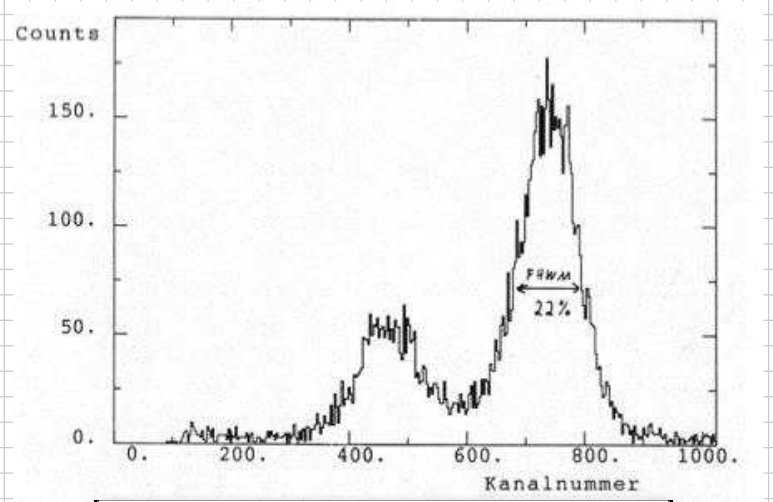
\includegraphics[width=0.5\textwidth]{5-escapePeak.jpg}
	\caption{Beispiel: Test von Proportionalkammern mit einem $^{55}$Fe-Präparat, Linie bei
	$5{,}89\,$keV. Photonen werden im Argongas der Kammer absorbiert, wodurch unterhalb des Photopeaks
	bei etwa $2{,}9\,$keV ein Escape-Peak auftritt.
	}
	\label{escapepeak}
\end{figure}
